\RequirePackage[hyphens]{url}
\documentclass [11pt, a4paper, twocolumn]{article}

\usepackage[slovak]{babel}
\usepackage{times}
\usepackage[utf8]{inputenc}
\usepackage{hyperref}
\usepackage{graphicx}
\usepackage[center]{caption}
\usepackage{float}
\usepackage{enumitem}
\usepackage{subcaption}
\captionsetup{compatibility=false}
\usepackage[left=1.5cm, text={18cm, 25cm}, top = 2.5cm]{geometry}
\setlength{\parskip}{0em}
\setlist[itemize]{noitemsep, topsep=0pt}

\begin{document}

\title{Interaktívna segmentácia obrazu pomocou Inside-Outside Guidance}
\author{Sabína Gregušová, Jan Šamánek, Adrián Tulušák\\xgregu02, xsaman02, xtulus00}
\date{}
\maketitle

\section{Úvod}
V posledných rokoch sa začali rapídne rozvíjať práce zamerané na segmentáciu obrazu. Tento typ úlohy má potenciál nájsť uplatnenie v rôznych odvetviach, menovito v samoriadiacich vozidlách, analýze medicínskych či vzdušných snímkov, alebo v editácii videí či fotiek, a mnohých iných. Zaujímavou podúlohou pre segmentáciu obrazu je práve interaktívna segmentácia obrazu. Cieľom všeobecnej segmentácie je identifikovať a vysegmentovať všetky objekty v obraze na základe príslušnej triedy, zatiaľ čo interaktívna segmentácia sa zameriava na oddelenie jedného, užívateľom vybraného objektu \textit{(foreground)}, od všetkého ostatného v obraze \textit{(background)}.

\subsection{Existujúce riešenia}
Jedným z prvých algoritmov, ktorý využíval deep-learning algoritmus bol \textit{Deep Interactive Object Selection} pre interaktívnu segmentáciu obrazu predstavený v \cite{xu_price_cohen_yang_huang_2016}. Tento článok jednoducho zhŕňa aj všetky predchádzajúce prístupy, napríklad dovtedy najznámejší \cite{boykov_jolly}, ktorý využíval algoritmus \textit{Interactive Graph Cut}, na ktorý ďalej naviazali v článku \cite{rother_kolmogorov_blake_2004} s optimalizovanou iteratívnou verziou. Tieto staršie algoritmy však veľmi záviseli na kvalite a hlavne množstve užívateľského vstupu, zatiaľ čo algoritmus \textit{Deep Interactive Object Selection} veľmi zredukoval požadované množstvo užívateľského vstupu. Za užívateľský vstup prijímal \textit{negatívne} (tam, kde sa objekt nachádza) a \textit{pozitívneho} kliknutia (tam, kde sa objekt nenachádza), ktoré boli ďalej transformované do \textit{Euklidovských distance máp}. Tento model bol natrénovaný pomocou FCN siete a dosahoval IoU až okolo $85\%$ pri viac ako 6 kliknutiach.

Hoci tento algoritmus dosahoval dobré metriky, minimálne 6 kliknutí je pre bežného užívateľa  stále dosť. Tento problém sa snaží riešiť algoritmus \textit{Inside-Outside Guidance} v \cite{zhang_liew_wei_wei_zhao_2020}, ktorý môžeme považovať za jeden zo State-of-the art systémov, a na tomto prístupe je založená aj naša implementácia projektu.

\section{Metóda}
Náš tím si zvolil prístup \textit{Inside-Outside Guidance} (dalej iba IoG) \cite{zhang_liew_wei_wei_zhao_2020}, ktorého hlavným cieľom je zredukovať množstvo užívateľského vstupu a dosahovať metriky porovnateľné s predchádzajúcimi existujúcimi riešeniami. Podstatou IOG je najskôr získať \textit{bounding box} pomocou dvoch kliknutí užívateľa (buď dvojica \textit{horný ľavý roh, dolný pravý roh} alebo \textit{horný pravý roh, dolný ľavý roh}) a zvyšné dve chýbajúce súradnice tohto obĺžnika je možné dopočítať. Užívateľ ďalej umiestni jedno kliknutie do vnútra objektu, ktorý chce vysegmentovať. Tento prístup ďalej umožňuje pridávať kliknutia aj po segmentácii obrazu a spresňovať ju, ak s ňou užívateľ nie je spokojný. Výhodou je, že bounding box nemusí úplne tesne obklopovať vybraný objekt. Kliknutia sú následne reprezentované ako v článku \cite{maninis} pomocou \textit{heatmapy}, kde bounding box predstavuje jednu heatmapu a zvyšné kliknutia druhú. Pri štandardnom RGB obrázku má teda výsledný obrázok 5 kanálov (3 pre RGB a 2 pre heatmapy).

\begin{figure}[H]
\centering
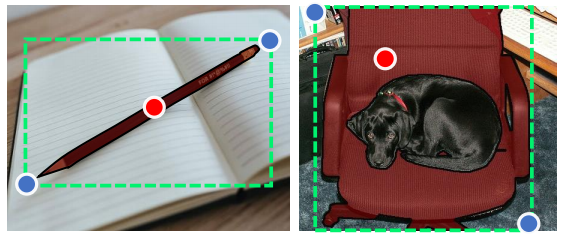
\includegraphics[width=\linewidth]{IoG}
\caption{Ukážka použitia prístupu \textit{Inside-Outside Guidance} pre užívateľský vstup. Prevzaté z \cite{zhang_liew_wei_wei_zhao_2020}.}
\end{figure}

Pri trénovaní siete nie je reálné, aby bol vstup získaný od skutočného užívateľa, ale musí byť náhodne vzorkovaný. Toto je implementované výberom bounding boxu z anotácie obrázku, ku ktorému je pripočítaný náhodný šum, aby vstup vyzeral ako od skutočného užívateľa. Kliknutie vo vnútri objektu je náhodne vygenerované vo vnútri objektu, s paddingom od okraja bounding boxu. Najväčšou výhodou tohto prístupu je schopnosť generalizovať aj iný typ predtým nevidených obrázkov bez potreby finetunovania.  

\section{Dataset}
Momentálne existujú mnohé dostupné datasety určené pre segmentáciu obrazu, ktoré sa dajú adaptovať aj na interaktívnu segmentáciu. Medzi najčastešie používané patrí \textit{Pascal}, \textit{Grabcut}, \textit{Berkley} alebo \textit{MS Coco}; a sú najčastejšie používané pre validáciu a porovnanie presnosti medzi dnešnými state-of-the-art systémami.

Pre náš projekt sme sa rozhodli použiť dataset \textit{MS Coco} pre evaluáciu aj trénovanie, pretože obsahuje cez 80 objektov vo viac ako 200 000 obrázkoch, ktoré zachytávajú bežné objekty zo života. Pre projekt bol použitý trénovací a validační dataset z roku 2017. Tento trénovací dataset obsahuje okolo 20 GB dát, ale pri trénovaní sa používala pravidelne obmieňaná polovica tohto datasetu kvôli obmedzeným výpočetným prostriedkom.

\begin{figure}[H]
\centering
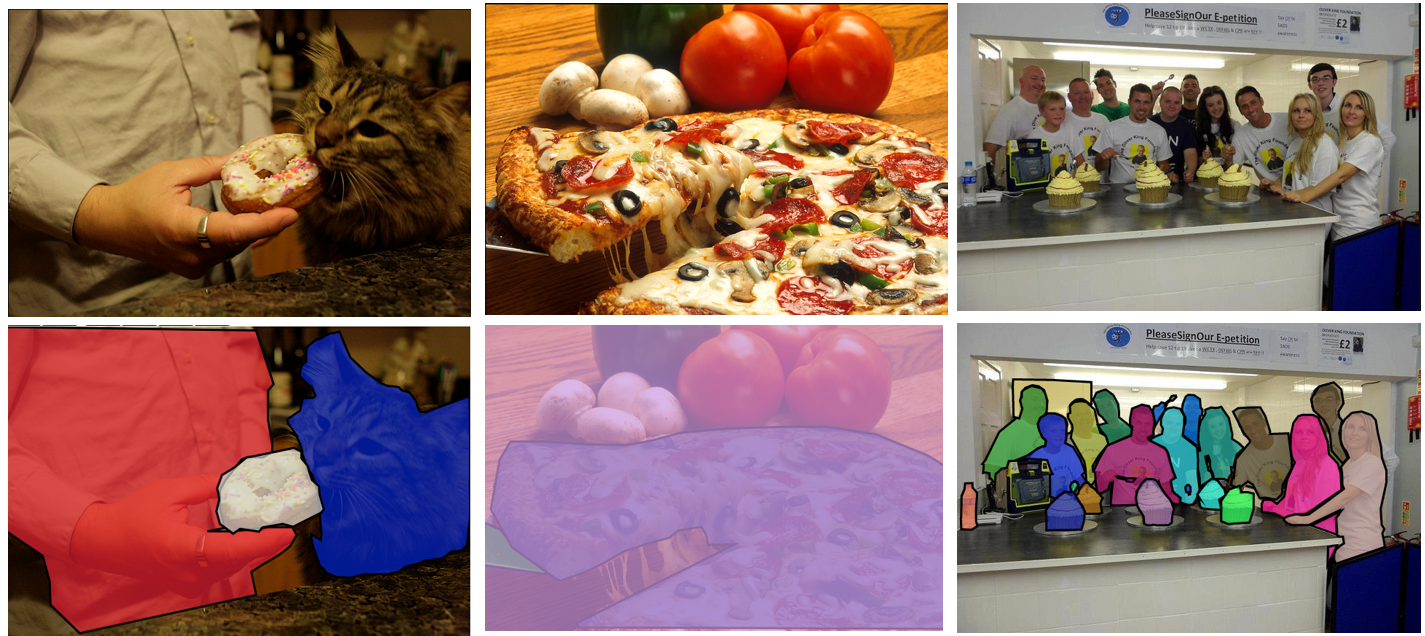
\includegraphics[width=\linewidth]{coco}
\caption{Ukážka obrázkov z datasetu \textit{MS Coco}. \\Prevzaté z \cite{coco}.}
\end{figure}

\section{Model}

Model pre túto úlohu je založený na dvoch podsieťach: \textit{CoarseNet} a \textit{FineNet}. Takáto architektúra bola pôvodne navrhnutá pre odhadnutie pózy človeka v obrázku. 

\begin{figure}[H]
\centering
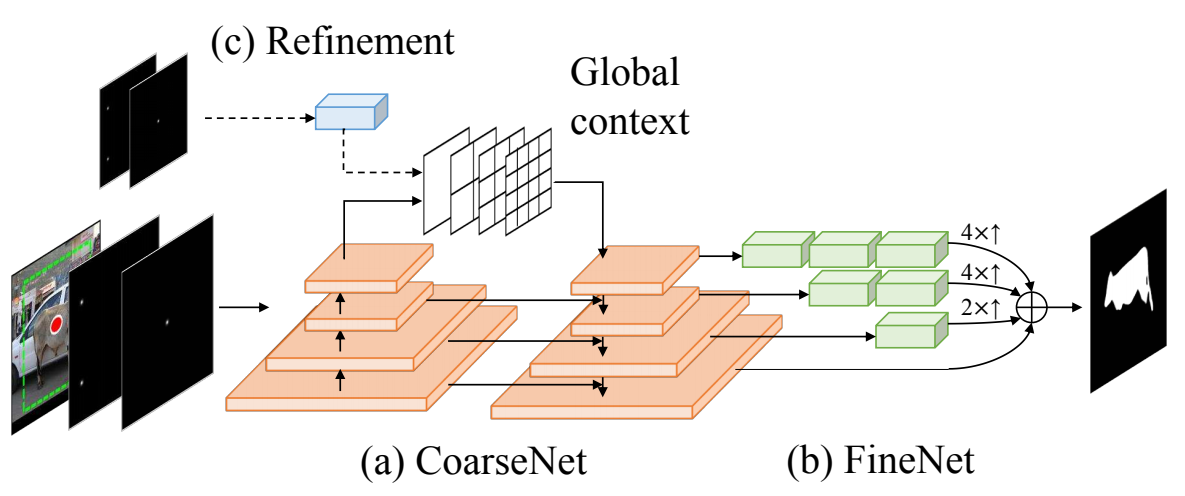
\includegraphics[width=\linewidth]{architecture}
\caption{Ukážka konceptu architektúry pre tento typ úlohy. Prevzaté z \cite{zhang_liew_wei_wei_zhao_2020}.}
\end{figure}


\textit{CoarseNet} má v našom prípade upravenú architektúru veľmi podobnú \textit{Resnet-50}, usporiadanej do pyramídovej štruktúry. Takáto sieť postupne aplikuje konvolúcie na vstupný batch obrázkov, na najhlbšej vrstve môže pridať \textit{refinement heatmapu} pre globálny kontext. Následne na najhlbšej vrstve aplikuje dekonvolúciu, až kým sa nedostane na pôvodnú veľkosť batchu obrázku. Ako aktivačná funkcia pre všetky vrstvy je použitá ReLU.

\textit{FineNet} je použitá na upsamplovanie medzivrstiev \textit{CoarseNetu}, ktoré sú následne skonkatenované a tvoria výstupný obrázok. Jej cieľom je obnoviť chýbajúce detaily, ako napríklad hranice objektu. \textit{FineNet} taktiež využíva ReLU na všetkých vrstvách okrem poslednej, kde je kvôli tresholdovaniu použitá sigmoida.

Pri trénovaní bol použitý learning rate s hodnotou $0.001$, optimalizátorom \textit{Adam} a chybová funkcia pre binárnu cross-entropiu.

\section{Evaluácia}
Po každej epoche trénovania bol model evaluovaný na základe 3 metrík (\cite{tiu_2020}):

\begin{itemize}
\item \textit{Pixel accuracy} - porovnáva, či sa jednotlivé pixely rovnajú; avšak táto metrika môže byť zavádzajúca, ak sú triedy na obrázku v nerovnováhe
\item \textit{Intersection over union (IoU)} - metrika, ktorá delí prienik očakávaného obrázku a predikcie modelu s ich zjednotením; najčastejšie používaná metrika pre porovnanie systémov
\item \textit{Dice coefficient} - metrika, ktorá používa dvojnásobok prieniku očakávaného obrázku a predikcie modelu podelený plochou oboch obrázkov v pixeloch 
\end{itemize}
Experimentálne boli implementované všetky 3 metriky, avšak pre výber najlepšieho modelu bola použitá metrika IoU, keďže väčšina systémov používa práve túto metriku pre prezentáciu výsledkov.



Celkovo bol model natrénovaný pomocou 21 generácií. Výsledky boli pozitívne:

\begin{figure}[H]
\centering
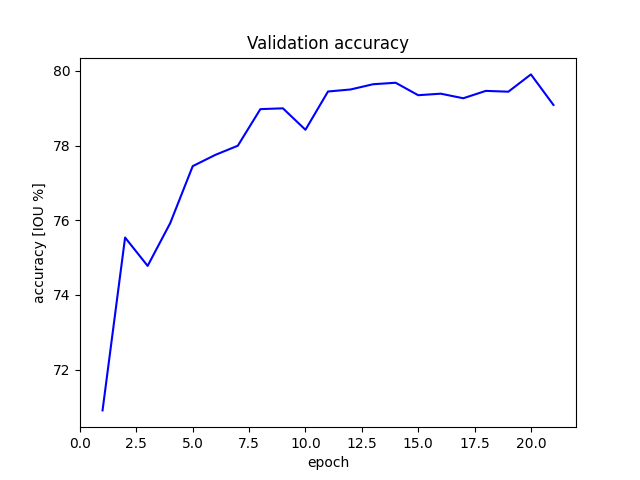
\includegraphics[width=\linewidth]{val_accuracy}
\caption{Priebeh validačnej metriky IoU počas všetkých generácií trénovania}
\end{figure}

Ostatné metriky dosiahli taktiež dobrých výsledkov:

\begin{center}
\begin{tabular}{|c| c|}
\hline
\textbf{Metrika} & \textbf{Ohodnotenie}\\ \hline
Pixel accuracy & 92.307\% \\ \hline
IoU & 79.904\% \\ \hline
Dice Coefficient & 88.829\% \\
\hline
\end{tabular}
\end{center}

Pôvodný článok pre IOG dosahoval približne $90\%$ pre IoU, avšak je potrebné dodať, že využíval ako backbone \textit{Resnet-101}, čo je sieť 2x tak veľká, ako bola použitá v tomto projekte, preto môžeme považovať IoU blížiace sa k $80 \%$ za veľmi slušný výsledok.

Nasledujúca ukážka prezentuje zobár vstupných obrázkov v RGB, vybraný bounding box, náhodne vygenerované kliknutie vo vnútri objektu, očakávaná segmentácia, predikcia modelu bez thresholdovania a predikcia modelu thresholdovaná na rôznych hodnotách. Vo finále je predikcia thresholdovaná na hodnote $0.5$.

\begin{figure}[H]
\centering
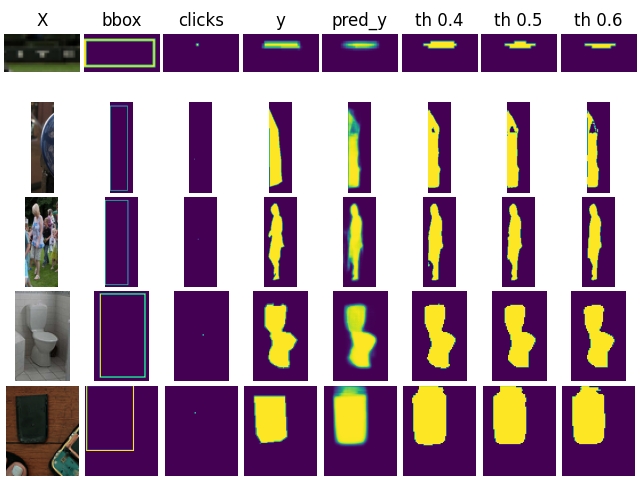
\includegraphics[width=\linewidth]{results3}
\caption{Vizualizácia výsledkov segmentácie z nášho natrénovaného modelu.}
\end{figure}

\section{Praktická aplikácia a GUI}

Vrámci projektu bolo implementované jednoduché užívateľské rozhranie v jazyku \texttt{Python} pomocou modulu \texttt{tkinter}. Toto rozhranie umožňuje priamu interakciu skutočného užívateľa s obrázkom. Užívateľ si vyberie ľubovolný obrázok zo svojho pevného disku, pravým tlačítkom myši môže užívateľ umiestniť bounding box. Keďže sa môže na obrázku nachádzať iba jeden bounding box, po opätovnom kliknutí pravého tlačítka sa začne kresliť nový bounding box. Ľavým tlačítkom sa umiestňujú kliknutia vo vnútri objektu a užívateľ môže urobiť ľubovolne veľa kliknutí. Spravidla je segmentácia s väčším množstvom kliknutí presnejšia, najmä pri objektoch s nerovnomerným tvarom. Ak užívateľ urobil chybu v kliknutiach, môže ich zmazať tlačítkom \texttt{Reset Clicks}. Po zadaní užívateľského vstupu stačí stlačiť tlačidlo \texttt{Segment} a počkať na výsledok.

Na hardvéri s horším CPU je to rádovo pár sekúnd, pri veľmi veľkom obrázku to môže byť až niekoľko desiatok sekúnd. Ak počítač obsahuje aj GPU, tak je výpočet značne rýchlejší a trvá pár milisekúnd až sekúnd.

\begin{figure}[H]
\centering
\begin{minipage}[H]{0.75\linewidth}
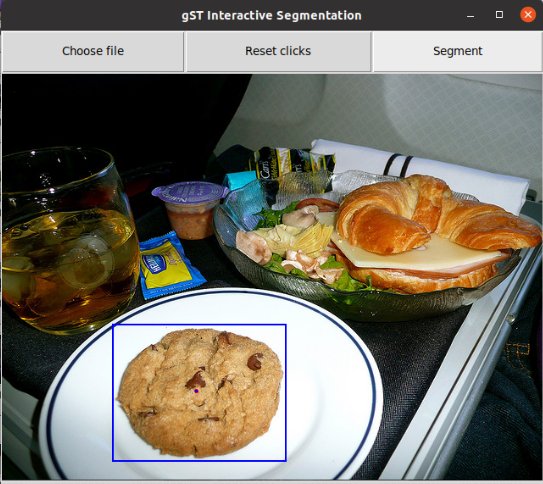
\includegraphics[width=\linewidth]{cookie_GUI_bef}
\caption{Obrázok s vybraným užívateľským vstupom}
\end{minipage}
\quad
\begin{minipage}[H]{0.75\linewidth}
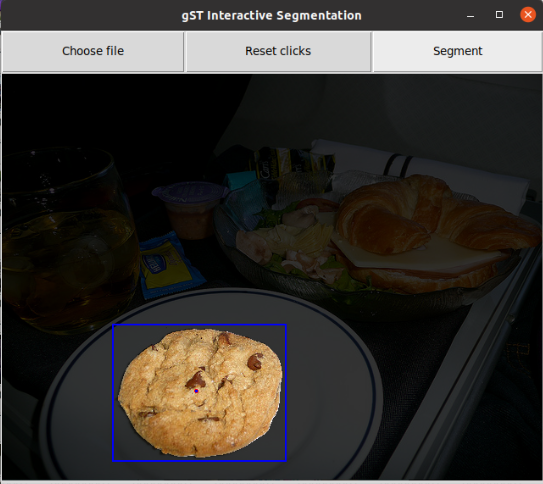
\includegraphics[width=\linewidth]{cookie_GUI}
\caption{Výsledok segmentácie nášho najlepšieho modelu trénovaného 20 generácií}
\end{minipage}
\end{figure}

\section{Ďalšie smery výskumu}
Ak by boli pre trénovanie dostupné lepšíe výpočetné zdroje, mohla by byť \textit{CoarseNet} zmenená z \textit{Resnet-50} na hlbšiu sieť \textit{Resnet-101}, ktorá by síce vyžadovala ovela dlhšie trénovanie, ale pravdepodobne by dosahovala presnosť porovnateľnú so sieťou z pôvodného článku. Zároveň by v budúcnosti mohla byť validácia rozšírená aj na iné dostupné datasety, vrátane obrázkov, ktoré obsahujú predtým nevidené objekty.


\newpage

\bibliographystyle{czechiso}
\renewcommand{\refname}{Použitá literatúra}
\bibliography{bibliography}

\end{document}